\documentclass[a4paper,12pt]{article}
\usepackage{titling}
\usepackage[OT4]{fontenc}
\usepackage[english,polish]{babel}
\usepackage{amsmath, amsfonts, amsthm, latexsym}

% Margins in document
\usepackage[left=2.5cm, right=2.5cm, top=3.5cm]{geometry}

% Indentation at the beginning of chapters/sections
\usepackage{indentfirst}

% Ceiling functions
\usepackage{mathtools}
\DeclarePairedDelimiter{\ceil}{\lceil}{\rceil}

% Avoid  colons before tables' empty captions and change caption
\usepackage{caption}
\captionsetup[table]{name=Tab.}
\captionsetup[figure]{name=Rys.}

% Don't know why, it starts from 2
\addtocounter{table}{0}

% Rename tables' suffix
\renewcommand{\tablename}{Tab.}

% Graphicx setup
\usepackage{graphicx}
\graphicspath{{graphics/}{../graphics/}}

% No separator between items
\usepackage{enumitem}
\setlist{nolistsep}

% Pagebreak before every \section
\let\oldsection\section
\renewcommand\section{\clearpage\oldsection}

% Bigger padding in tabulars
\usepackage{array}
\setlength\extrarowheight{3pt}

% Itemize in tabulars (avoid big margins with minipage)
\newcommand{\tabbeditemize}[1]{
	\begin{minipage}[t]{0.4\textwidth}
		\begin{itemize}[topsep=0mm,partopsep=0mm,leftmargin=4mm]
			#1
		\end{itemize}
\end{minipage}}

% listings
\usepackage{xcolor}
\usepackage{listings}
\usepackage{hyperref}
\definecolor{codegreen}{rgb}{0,0.7,0}
\definecolor{codegray}{rgb}{0.5,0.5,0.5}
\definecolor{codepurple}{rgb}{0.58,0,0.82}
\definecolor{backcolour}{rgb}{0.95,0.95,0.92}
\lstdefinestyle{mystyle}{
	language=Python,
	deletekeywords={from},
	backgroundcolor=\color{backcolour},   
	commentstyle=\color{codegreen},
	keywordstyle=\color{magenta},
	numberstyle=\tiny\color{codegray},
	stringstyle=\color{codepurple},
	basicstyle=\ttfamily\footnotesize,
	breakatwhitespace=false,         
	breaklines=true,                 
	captionpos=b,                    
	keepspaces=true,                 
	numbers=left,                    
	numbersep=5pt,                  
	showspaces=false,                
	showstringspaces=false,
	showtabs=false,                  
	tabsize=4
}

% Nazwa gry
\newcommand{\nazwagry}{\textit{Domineering}}

% DOCUMENT
\title{
	Zastosowanie algorytmu UCT do stworzenia sztucznej inteligencji grającej w \nazwagry\\
	\large Wstępna dokumentacja projektu}

\author{Patryk Fijałkowski \\ Mateusz Burczaniuk}

% ============================================
% CONTENT ====================================
% ============================================

\begin{document}
\begin{titlingpage}
	\maketitle
	\vspace{3cm}
\end{titlingpage}


\section{Opis \nazwagry}
TODO

\section{Algorytmy MCTS}
Monte-Carlo Tree Search to heurystyka, której celem jest podejmowanie decyzji w pewnych zadaniach sztucznej inteligencji, na przykład wybieranie ruchów w grach. Metoda jest oparta na przeszukiwaniu możliwych stanów gry zapisanych w wierzchołkach drzewa i losowym symulowaniu rozgrywek. Algorytmy MCTS opierają się na rozbudowywaniu drzewa ze stanami gry przez iteracyjne wykonywanie czterech faz. Jednym z najpowszechniejszych wariantów MCTS jest algorytm UCT. Pseudokod opisany w Listingu \ref{lst:mcts} oraz implementacja MCTS w projekcie bazują na \cite{banditbased}. Przykład działania algorytmu ze szczególnym uwzględnieniem kolejnych faz znajduje się na Rysunku \ref{rys:mcts_phases}.

\begin{figure}[h]
	\centering
	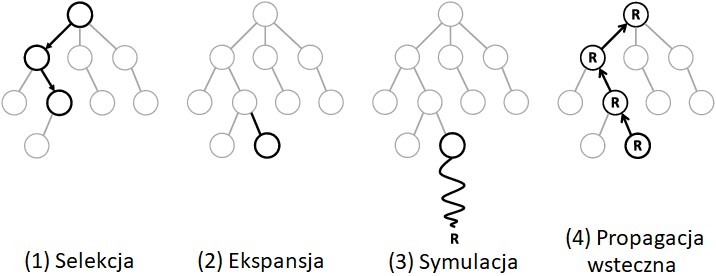
\includegraphics[width=0.8\textwidth]{mcts_phases_pl.png}
	\caption{Fazy MCTS, źródło: \cite{mctsanalysis}}
	\label{rys:mcts_phases}
\end{figure}

\begin{enumerate}
	\item \textbf{Faza selekcji} (wiersz 6 w listingu) -- wybór pewnego liścia drzewa. Rozdział \ref{subsec:uct} opisuje jeden ze sposobów na wybranie wierzchołka w tej fazie.
	\item \textbf{Faza ekspansji} (wiersz 7 w listingu) -- utworzenie wierzchołków potomnych dla wierzchołka wybranego w fazie selekcji. Tworzone wierzchołki odpowiadają stanom możliwym do uzyskania przez wykonanie jednego ruchu ze stanu rodzica.
	\item \textbf{Faza symulacji} (wiersz 10 w listingu) -- rozegranie partii składającej się z losowych ruchów ze stanu jednego z wierzchołków utworzonych w poprzedniej fazie. Rozgrywana jest ona do końca, czyli do wyłonienia zwycięzcy lub spowodowania remisu, lub jest ucinana po pewnej liczbie ustalonych ruchów i wynik gry jest ewaluowany przez pewną funkcję.
	\item \textbf{Faza propagacji wstecznej} (wiersz 11 w listingu) -- aktualizacja informacji na temat wierzchołków na ścieżce od liścia, z którego rozpoczęto symulację, do korzenia drzewa. Główną przekazywaną wartością jest wynik symulacji.
\end{enumerate}

\begin{minipage}{\linewidth} % minipage to ensure listing is on seperate page
	\begin{lstlisting}[caption={Pseudokod algorytmu Monte Carlo Tree Search}, label=lst:mcts, style=mystyle]
def find_next_move(curr_state):
	iterations_counter = 0
	tree = initialize_tree(curr_state)
	
	while iterations_counter < max_iterations_counter:
		curr_node = select a leaf from tree
		create child nodes from curr_node
		if curr_node has children:
			curr_node = random child of curr_node
		playout_result = simulate random playout from curr_node     
		update tree according to playout_result                     
		iterations_counter++
	
	best_state = select best child(tree.root) 
	return best_state
	\end{lstlisting}
\end{minipage}


\subsection{Algorytm UCT} \label{subsec:uct}
UCT jest wariantem metody MCTS, który stara się zachować równowagę między eksploatacją bardziej obiecujących ruchów a eksploracją tych rzadko odwiedzonych. Formuła, która odpowiada za wyznaczenie najbardziej obiecującego wierzchołka w fazie wyboru MCTS jest przedstawiona jako wyrażenie (\ref{formula:uct}).

\begin{equation}\label{formula:uct}
\frac{w_i}{n_i} + c \sqrt{\frac{\ln N_i}{n_i}}
\end{equation}

W wyrażeniu (\ref{formula:uct}), indeks $i$ odnosi się do liczby wykonanych przez algorytm iteracji, czyli czterech faz MCTS. W pierwszym składniku sumy wyrażenia (\ref{formula:uct}), licznik $w_i$ oznacza sumę wszystkich wypłat w danym węźle, a mianownik $n_i$ oznacza liczbę rozegranych symulacji. Zatem ułamek ten przyjmuje wartości większe dla ruchów o większej średniej wygranej, co odpowiada ze eksploatację drzewa. Drugi składnik sumy wyrażenia (\ref{formula:uct}) przyjmuje wartości większe dla wierzchołków, dla których wykonano mniej symulacji i odpowiada eksploracji drzewa. $N_i=\sum_i n_i$, a $c$ jest parametrem eksploracji, który może być dostosowany do badanego problemu.


\subsection{Algorytm PUCT} 
TODO


\subsection{Algorytm UCT - wariant 2}
TODO


\section{Algorytm zachłanny}
TODO



\section{Rozwiązanie}


\section{Hipotezy badawcze}



\section{Harmonogram działań}
W tabeli \ref{tab:schedule} przedstawiono planowany harmonogram działań podczas pracy nad projektem.

\begin{table}[h!]
	\centering
	\caption{Harmonogram pracy}
	\label{tab:schedule}
	\smallskip
	\begin{tabular}{|l|l|}
		\hline
		\textbf{Deadline}   & \textbf{Przygotowane zadania} \\ \hline
		
		06.05.2020 	& Stworzenie dokumentacji projektu \\ 
		& Zaimplementowanie struktur potrzebnych do operowania na drzewach \\ \hline
		
		13.05.2020  & Zaimplementowanie logiki gry \\
		& Przygotowanie aplikacji okienkowej \\ \hline
		
		20.05.2020	& Zaimplementowanie algorytmu UCT  \\ \hline
		
		07.05.2020	&  Zaimplementowanie algorytmu heurystycznego \\ 
		& Zaimplementowanie dwóch wariantów UCT \\ \hline
		
		03.06.2020	& Przeprowadzenie eksperymentów w celu weryfikacji hipotez \\ 
		&  Wstępna weryfikacja postawionych hipotez \\ \hline
		
		10.06.2020	& Pełna weryfikacja postawionych hipotez \\ 
		& Stworzenie raportu \\ \hline
	\end{tabular}
\end{table}


\section{Projekt techniczny}
Projekt zostanie sporządzony przy użyciu języka C\#. Nie jest planowane użycie żadnych specjalistycznych bibliotek tego języka.

\begin{thebibliography}{20}
	\bibitem[1]{banditbased} Levente Kocsis, Csaba Szepesvári, \emph{Bandit based Monte-Carlo Planning}, European Conference on Machine Learning, Berlin, Germany, September 18--22, 2006.
	\bibitem[2]{mctsanalysis} Steven James, George Konidaris, Benjamin Rosman, \emph{An Analysis of Monte Carlo Tree Search}, University of the Witwatersrand, Johannesburg, South Africa.
	\bibitem[3]{tron} Pierre Perick, David L. St-Pierre, Francis Maes, Damien Ernst, \emph{Comparison of Different Selection Strategies in Monte-Carlo Tree Search for the Game of Tron},  IEEE Conference on Computational Intelligence and Games, Granada, Spain, September 12--15, 2012.
	 %http://www.montefiore.ulg.ac.be/~dlstpierre/publications/tron2012.pdf
\end{thebibliography}

\end{document}
